\documentclass[10pt]{beamer}
\usetheme{Madrid}
\usepackage{booktabs}
\usepackage{multirow}
%\usepackage{sidecap}
%\usepackage[style=authoryear]{biblatex}
\usecolortheme{seahorse}
%\usefonttheme{professionalfonts}
\setbeamertemplate{footline}
        {
      \leavevmode%
      \hbox{%
      \begin{beamercolorbox}[wd=.333333\paperwidth,ht=2.25ex,dp=1ex,center]{author in head/foot}%
        \usebeamerfont{author in head/foot}\insertshortauthor~~(\insertshortinstitute)
      \end{beamercolorbox}%
      \begin{beamercolorbox}[wd=.333333\paperwidth,ht=2.25ex,dp=1ex,center]{title in head/foot}%
        \usebeamerfont{title in head/foot}\insertshorttitle
      \end{beamercolorbox}%
      \begin{beamercolorbox}[wd=.333333\paperwidth,ht=2.25ex,dp=1ex,right]{date in head/foot}%
        \usebeamerfont{date in head/foot}\insertshortdate{}\hspace*{2em}

    %#turning the next line into a comment, erases the frame numbers
        %\insertframenumber{} / \inserttotalframenumber\hspace*{2ex} 

      \end{beamercolorbox}}%
      \vskip0pt%
    }
%\mode<presentation>
%\usepackage{beamerthemesplit}
\usepackage{multimedia}
\usepackage{hyperref}
\usepackage{tabularx}
\usepackage{animate}
%\usepackage{mathtools}

%\beamertemplateballitem
\setbeamertemplate{navigation symbols}{}

\usepackage{amsfonts, amsmath, graphicx,color}

\newcommand{\prob}{\mathbb{P}}                  % probability
\newcommand{\E}{\mathbb{E}}											% expectation
\newcommand{\F}{\mathcal{F}}
\newcommand{\Fz}{\mathcal{F}^{(Z)}}
\newcommand{\Fc}{\mathcal{F}^{(C)}}
\newcommand{\R}{\mathbb{R}}
\newcommand{\Z}{\mathcal{Z}}
\newcommand{\N}{\mathcal{N}}
\newcommand{\Ss}{\mathbb{S}}
\newcommand{\bz}{\mathbf{z}}
\newcommand{\norm}{\mathcal{N}}
\newcommand{\Cset}{\mathcal{C}}
\newcommand{\Ctrans}{\mathcal{C}_{\text{trans}}}
\newcommand{\Cposs}{\mathcal{C}_{\text{poss}}}
\newcommand{\Cend}{\mathcal{C}_{\text{end}}}

\newenvironment{Cpossdef}[1][Ball Possession States]{\begin{trivlist}
	\item[\hskip \labelsep {\bfseries #1}]}{\end{trivlist}}
\newenvironment{Cenddef}[1][End States]{\begin{trivlist}
	\item[\hskip \labelsep {\bfseries #1}]}{\end{trivlist}}
\newenvironment{Ctransdef}[1][Transition States]{\begin{trivlist}
	\item[\hskip \labelsep {\bfseries #1}]}{\end{trivlist}}



\newcommand{\Cmap}{\mathscr{C}}
\newcommand{\bTh}{\boldsymbol{\Theta}}

%\newtheorem{theorem}{Theorem}[section]
	%\newtheorem{lemma}[theorem]{Lemma}
	%\newtheorem{proposition}[theorem]{Proposition}
	%\newtheorem{corollary}[theorem]{Corollary}

	%\newenvironment{proof}[1][Proof]{\begin{trivlist}
	%	\item[\hskip \labelsep {\bfseries #1}]}{\end{trivlist}}
	%\newenvironment{definition}[1][Definition]{\begin{trivlist}
	%	\item[\hskip \labelsep {\bfseries #1}]}{\end{trivlist}}
	%\newenvironment{example}[1][Example]{\begin{trivlist}
	%	\item[\hskip \labelsep {\bfseries #1}]}{\end{trivlist}}
	%\newenvironment{remark}[1][Remark]{\begin{trivlist}
	%	\item[\hskip \labelsep {\bfseries #1}]}{\end{trivlist}}


\title[Multiresolution Basketball Modeling]{A Multiresolution Stochastic Process Model for Basketball Possession Outcomes}
\author[Dan Cervone]{Dan Cervone, Alex D'Amour, Luke Bornn, Kirk Goldsberry}
\institute[Harvard]{Harvard Statistics Department}
\date{August 11, 2015}

% Motivate data:
%  - gif of the game play, talk about how traditional statistics are confined to terminal events
%  - gif of data, then slide clearly describing data attributes + size of data
%  - these data allow us to quantify all movement, action, and decision-making
%  - EPV is our attempt to do this. The instantaneous expected point value of apossession given its evolution. EPV curves are possession "stock ticker"... one dimensional summaries of value.
%  - Much like stock prices are analyzed in behavioral economics, EPV curves can be analyzed for inferences on decision-making, strategy, spacing and positioning, etc.
% **** %
% Formally define EPV, stochastic process:
%  - EPV def
%  - Regression v markov v brute force
%  - Coarsened states, diagram from paper
%  - Stopping time definitions
%  - Assumptions, EPV theorem
% Multiresolution models:
%  - (M1)--(M4) (only talk about M1, M2)
%  - Micro model with chart
%  - Macro model with chart example
% Hierarchical modeling to share information across space and players... the Dwight Howard corner 3
%  - Player similarity adjacency matrix, and court basis functions
%  - Car prior for all model effects
%  - Estimation using INLA
% Results
%  - EPV curve
%  - EPVA, shot satisfaction
%  - Conclusion and future steps


\begin{document}

\frame{\titlepage}

\begin{frame}{NBA optical tracking data}
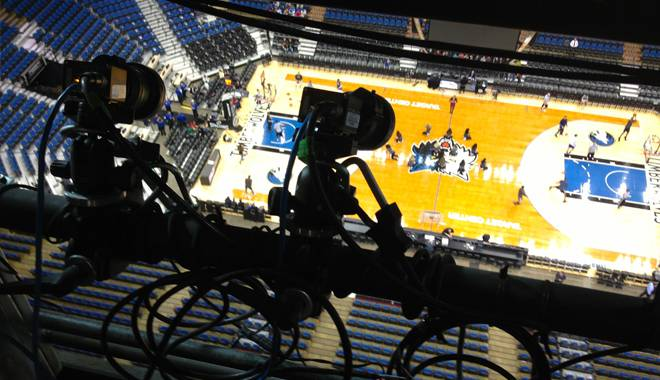
\includegraphics[width=1.0\textwidth]{graphics/sporvu.jpg}
% image of play-by-play data
% play video of possession
% play gif of possession
% explain potential here, all the information that's in non-terminal events
\end{frame}


\begin{frame}{NBA optical tracking data}
\begin{center}
\href{http://dcervone.com/wp-content/uploads/2015/01/nba_data.gif}{
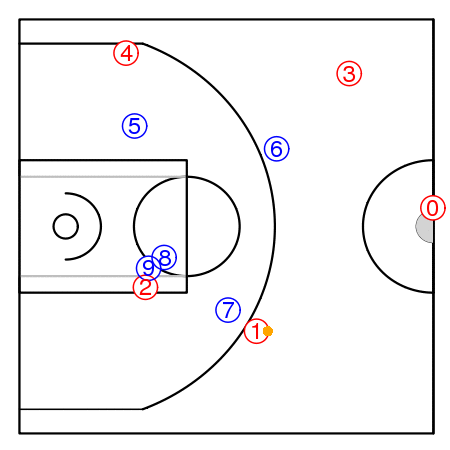
\includegraphics[scale=0.25]
{nba_data_frame}}
\end{center}
\pause
\vspace{-0.3cm}
\begin{itemize}
\item $(x,y)$ locations for all 10 players (5 on each team) at 25Hz.
\item $(x,y,z)$ locations for the ball at 25Hz.
\item Event annotations (shots, passes, fouls, etc.).
\item 1230 games from 2013-14 NBA, each 48 minutes, featuring 461 players in total.
\end{itemize}
\end{frame}

\begin{frame}{Expected Possession Value (EPV)}
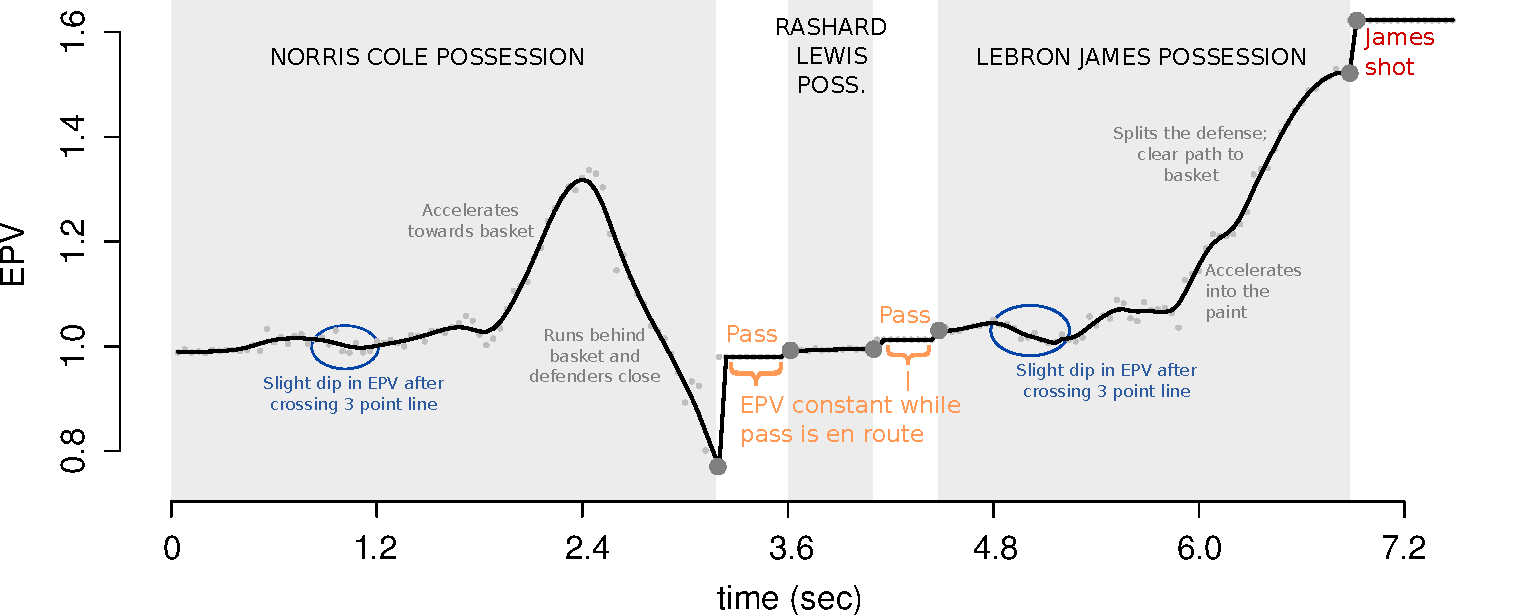
\includegraphics[width=1.0\textwidth]{graphics/ticker_1_edit}
\end{frame}

\begin{frame}{EPV definition}
Let $\Omega$ be the space of all possible basketball possessions. For $\omega \in \Omega$
\begin{itemize}
\pause 
\item $X(\omega) \in \{0, 2, 3\}$: point value of possession $\omega$.
\pause
\item $T(\omega)$: possession length
\pause
\item $Z_t(\omega), 0 \leq t \leq T(\omega)$: time series of optical tracking data.
\pause
\item $\Fz_t = \sigma(\{Z_s^{-1}: 0 \leq s \leq t\})$: natural filtration.
\end{itemize}
\pause
\begin{definition}
The \textit{expected possession value} (EPV) at time $t \geq 0$ during a possession is $\nu_t = \E[X|\Fz_t]$.
\end{definition}
\pause
\begin{itemize}
\item EPV provides an instantaneous snapshot of the possession's value, given its full spatiotemporal history.
\item $\nu_t$ is a Martingale: $\E[\nu_{t + h} | \Fz_t] = \nu_t$ for all $h > 0$.
\end{itemize}
\end{frame}

\begin{frame}{Calculating EPV}{$\nu_t = \E[X | \Fz_t]$}
Regression-type prediction methods:
\begin{itemize}
% \item Model points ($X$) versus possession features.
\item[--] Data are not traditional input/output pairs.
\item[--] No guarantee of stochastic consistency.
\end{itemize}
\pause
Markov chains:
\begin{itemize}
% \item Model spatially-discretized version of $Z_t$ as a homogeneous Markov chain.
\item[+] Stochastically consistent.
\item[--] Information is lost through discretization.
\item[--] Many rare transitions.
\end{itemize}
\pause
Brute force, ``God model'' for basketball.
\begin{itemize}
% \item $\prob(Z_{t + \epsilon} | \Fz_t)$ full-resolution transition Kernel.
\item[+] Allows Monte Carlo calculation of $\nu_t$ by simulating future possession paths.
\item[--] $Z_t$ is high dimensional and includes discrete events (passes, shots, turnovers).
\end{itemize}
\end{frame}
% cross through??

\begin{frame}{A coarsened process}
Finite collection of states $\Cset = \Cposs \cup \Cend \cup \Ctrans$.
%\vspace{-0.2cm}
\begin{columns}[T] % align columns
\begin{column}{.58\textwidth}
%\rule{\linewidth}{4pt}
%\rule{\linewidth}{1pt}
%\begin{center} \textbf{BALL POSSESSION STATES}
\begin{block}{$\Cposs$: Ball possession states}
\begin{center}
$\{\text{player}\} \times \{\text{region}\} \times \{\text{defender within 5 feet}\}$
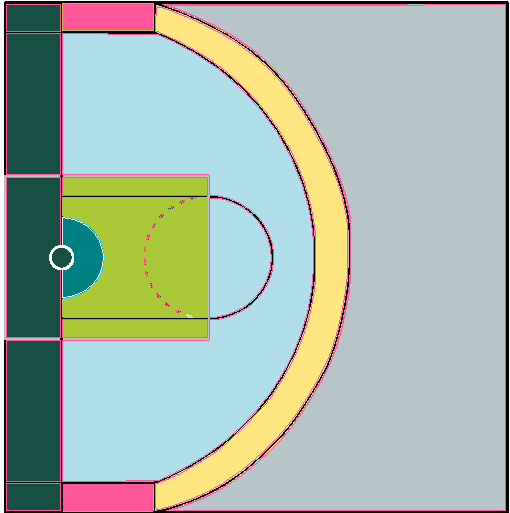
\includegraphics[scale=0.4]{graphics/court_cropped}
\end{center}
\end{block}
\end{column}%
%\vrule{}
\hfill%
\begin{column}{.4\textwidth}
\begin{minipage}{\textwidth}
%\hrule{}
\pause
\begin{block}{$\Cend$: End states}
\begin{center}
\{made 2, made 3, turnover\}
\end{center}
\end{block}
\end{minipage}
%\vskip12pt plus 1filll
\begin{minipage}{\textwidth}
%\hrule{}
\pause
\begin{block}{$\Ctrans$: Transition states}
\begin{center} \{\{ pass linking $c, c' \in \Cposs$\}, \{shot attempt from $c \in \Cposs$\}, turnover in progress, \\ rebound in progress \}.
\end{center}
\end{block}
\end{minipage}
\end{column}%
\end{columns}
\pause
\begin{itemize}
\item $C_t \in \Cset$: state of the possession at time $t$.
\item $C^{(0)}, C^{(1)}, \ldots, C^{(K)}$: discrete sequence of distinct states.
\end{itemize}
\end{frame}

\begin{frame}{Possible paths for $C_t$}
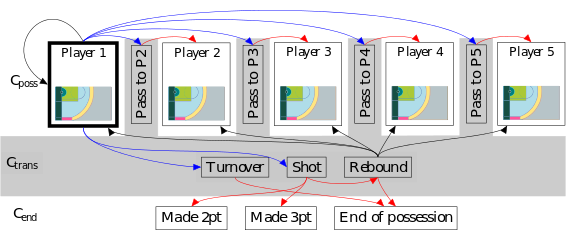
\includegraphics[trim=60 520 60 40,clip,width=\textwidth]{graphics/Ct_standalone}
\pause
\begin{align*}
\color{blue}{\tau_t} & = \begin{cases}
\text{min} \{ s : s > t, C_s \in \Cset_{\text{trans}}\} & \text{if } C_t \in \Cset_{\text{poss}} \\
t & \text{if } C_t \not \in \Cset_{\text{poss}}
\end{cases}  \\
\color{red} {\delta_t}  &= \text{min}\{s : s \geq \tau_t, C_s \not \in \Cset_{\text{trans}} \}.
\end{align*}

\end{frame}

\begin{frame}{Stopping times for switching resolutions}
\begin{align*}
\color{blue}{\tau_t} & = \begin{cases}
\text{min} \{ s : s > t, C_s \in \Cset_{\text{trans}}\} & \text{if } C_t \in \Cset_{\text{poss}} \\
t & \text{if } C_t \not \in \Cset_{\text{poss}}
\end{cases}  \\
\color{red} {\delta_t}  &= \text{min}\{s : s \geq \tau_t, C_s \not \in \Cset_{\text{trans}} \}.
\end{align*}
\pause
Key assumptions:
\begin{itemize}
\item[A1] $C$ is marginally semi-Markov.
\pause
\item[A2] For all $s > \delta_t$, $\prob(C_s | C_{\delta_t}, \Fz_t) = \prob(C_s | C_{\delta_t})$. 
\end{itemize}
\pause
\begin{theorem}
Assume (A1)--(A2), then for all $0 \leq t < T$, 
$$\nu_t = \sum_{c \in \{ \Ctrans \cup \Cend \}} \E[X | C_{\delta_t} = c]\prob(C_{\delta_t} = c | \Fz_t).$$
\end{theorem}
\end{frame}

\begin{frame}{Multiresolution models}
EPV:
$$\nu_t = \sum_{c \in \{ \Ctrans \cup \Cend \}} \E[X | C_{\delta_t} = c]\prob(C_{\delta_t} = c | \Fz_t).$$
\pause
Let $M(t)$ be the event $\{\tau_t \leq t + \epsilon\}$.
\begin{itemize}
\item[M1] $\prob(Z_{t + \epsilon} | M(t)^c, \Fz_t)$: the \emph{microtransition model}.
\item[M2] $\prob(M(t) | \Fz_t)$: the \emph{macrotransition entry model}.
\item[M3] $\prob(C_{\delta_t} | M(t), \Fz_t)$: the \emph{macrotransition exit model}.
\item[M4] $\mathbf{P}$, with  $P_{qr} = \prob(C^{(n+1)} = c_r | C^{(n)} = c_q)$: the \emph{Markov transition probability matrix}.
\end{itemize}
\pause
Monte Carlo computation of $\nu_t$:
\begin{itemize}
\item Draw $C_{\delta_t} | \Fz_t$ using (M1)--(M3).
\item Calculate $\E[X | C_{\delta_t}]$ using (M4).
\end{itemize}
\end{frame}

\begin{frame}{Microtransition model}
Player $\ell$'s position at time $t$ is $\mathbf{z}^{\ell}(t) = (x^{\ell}(t), y^{\ell}(t))$.
$$x^{\ell}(t + \epsilon) =  x^{\ell}(t) + \alpha^{\ell}_x[x^{\ell}(t) - x^{\ell}(t - \epsilon)] + \eta^{\ell}_x(t)$$
\begin{itemize}
\item $\eta^{\ell}_x(t) \sim \norm (\mu^{\ell}_x(\mathbf{z}^{\ell}(t)), (\sigma^{\ell}_x)^2)$.
\item $\mu_x$ has Gaussian Process prior.
\item $y^{\ell}(t)$ modeled analogously (and independently). 
\end{itemize}
\only<1>{\vspace{4.4cm}}

\pause
\only<2>{
\begin{center}
\begin{tabular}{cc}
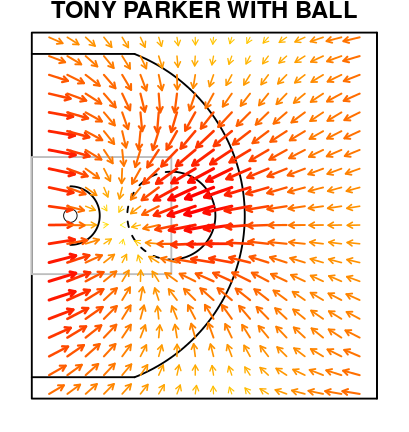
\includegraphics[scale=0.32]{graphics/parker_with} & 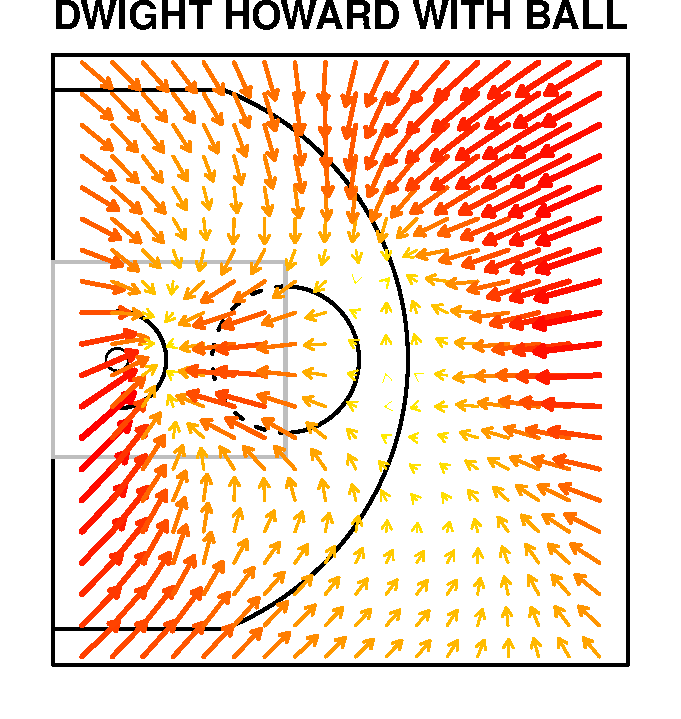
\includegraphics[scale=0.32]{graphics/howard_with}
\end{tabular}
\end{center}
}
\only<3->{
\begin{center}
\begin{tabular}{cc}
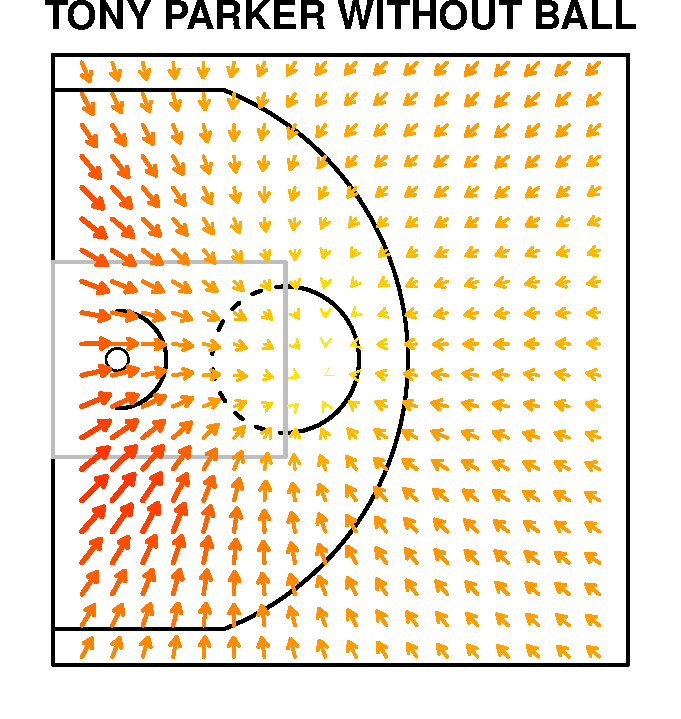
\includegraphics[scale=0.32]{graphics/parker_without} & 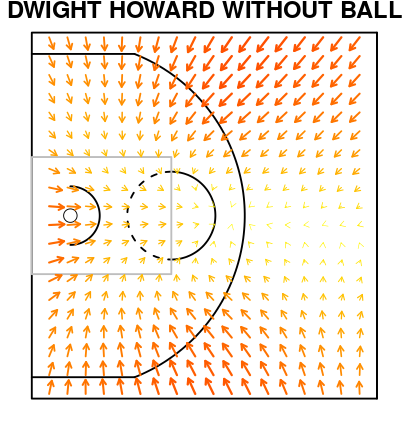
\includegraphics[scale=0.32]{graphics/howard_without}
\end{tabular}
\end{center}
}
\pause
\pause
\begin{itemize}
\item Defensive microtransition model based on defensive matchups \cite{franks2014defensive}.
\end{itemize}
\end{frame}

\begin{frame}{Macrotransition entry model}
Recall $M(t) = \{ \tau_t \leq t + \epsilon \}$:
\begin{itemize}
\item Six different ``types'', based on entry state $C_{\tau_t}, \cup_{j=1}^6 M_j(t) = M(t)$.
\item Hazards: $\lambda_j(t) = \lim_{\epsilon \rightarrow 0} \frac{\prob(M_j(t) | \Fz_t)}{ \epsilon}$.
\only<1-2>{
\begin{equation*}
\log(\lambda_j(t)) = [\mathbf{W}_j^{\ell}(t)]'\boldsymbol{\beta}_j^{\ell} + \xi_j^{\ell}\left(\bz^{\ell}(t)\right)
\end{equation*}
}
\only<3->{
\begin{equation*}
\log(\lambda_j(t)) = [\mathbf{W}_j^{\ell}(t)]'\boldsymbol{\beta}_j^{\ell} + \xi_j^{\ell}\left(\bz^{\ell}(t)\right) + \tilde{\xi}^{\ell}_j\left(\bz_j(t) \right)\mathbf{1}[j \leq 4]
\end{equation*}
}
\end{itemize}
\only<1>{\vspace{4.1cm}}
\only<2>{
\begin{center}
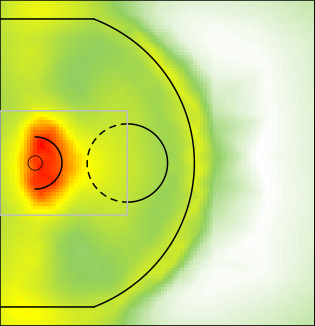
\includegraphics[scale=0.32]{graphics/lebron_take_spatial_2}
\end{center}
}
\only<3->{
\begin{center}
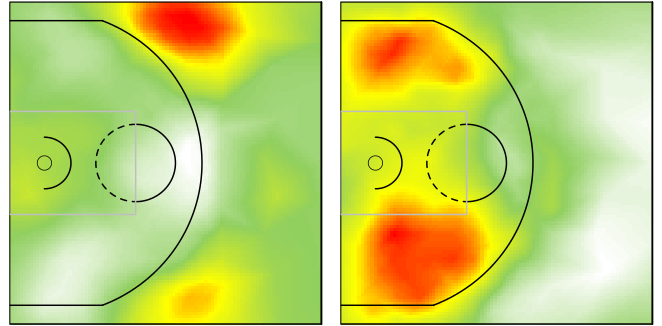
\includegraphics[scale=0.32]{graphics/lebron_pass4_spatial_2}
\end{center}
}
\end{frame}

\begin{frame}{Hierarchical modeling}
Dwight Howard's shot chart:
\begin{center}
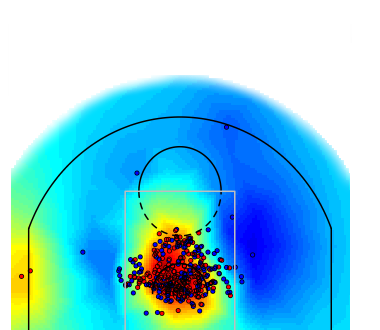
\includegraphics[width=0.75\textwidth]{graphics/howardshots1}
\end{center}
\end{frame}

\begin{frame}{Hierarchical modeling}
Shrinkage needed:
\begin{itemize}
\item Across space.
\item Across different players.
\end{itemize}
\begin{tabular}{cc}
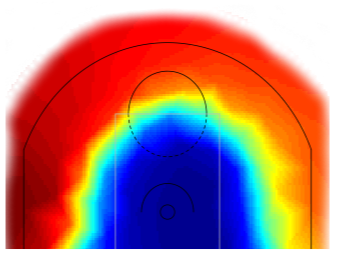
\includegraphics[width=0.45\textwidth]{graphics/shotspace2}
&
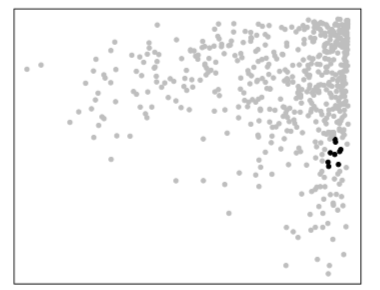
\includegraphics[width=0.45\textwidth]{graphics/howard_graph}
\end{tabular}
% Shrinkage space + player similarity
% computational details
% results
% epva / shot satis
\end{frame}

\begin{frame}{Basis representation of spatial effects}
Spatial effects $\xi^{\ell}_j$
\begin{itemize}
\item $\ell$: ballcarrier identity.
\item $j$: macrotransition type (pass, shot, turnover).
\end{itemize}
\pause
Functional basis representation
\begin{equation*}
\xi^{\ell}_j (\bz) = [\mathbf{w}^{\ell}_j]'\boldsymbol{\phi}_j(\bz).
\end{equation*}
\begin{itemize}
\item $\boldsymbol{\phi}_j = (\phi_{ji} \: \: \ldots \phi_{jd})'$: $d$ spatial basis functions.
\item $\mathbf{w}_j^{\ell}$: weights/loadings.
\end{itemize}
\pause
Information sharing
\begin{itemize}
\item $\boldsymbol{\phi}_j$ allows for non-stationarity, correlations between disjoint regions \cite{higdon2002space}.
\item $\mathbf{w}_j^{\ell}$: weights across players follow a CAR model \cite{besag1974spatial} based on player similarity graph $\mathbf{H}$.
\end{itemize}
\end{frame}

\begin{frame}{Basis representation of spatial effects}
Basis functions $\boldsymbol{\phi}_j$ learned in pre-processing step:
\begin{center}
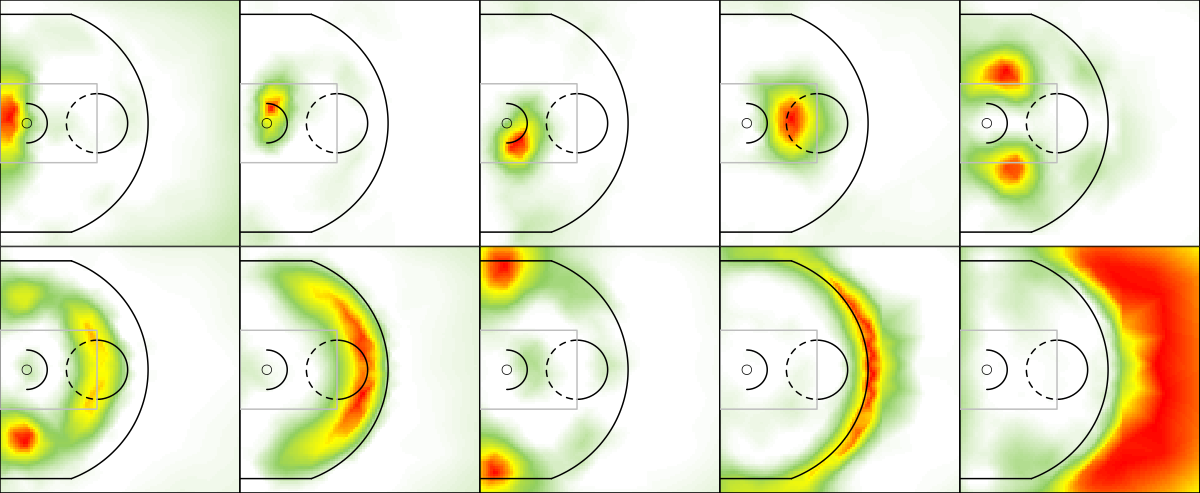
\includegraphics[width=0.7\textwidth]{graphics/bplots_3}
\end{center}
\pause
Graph $\mathbf{H}$ learned from players' court occupancy distribution:
\begin{center}
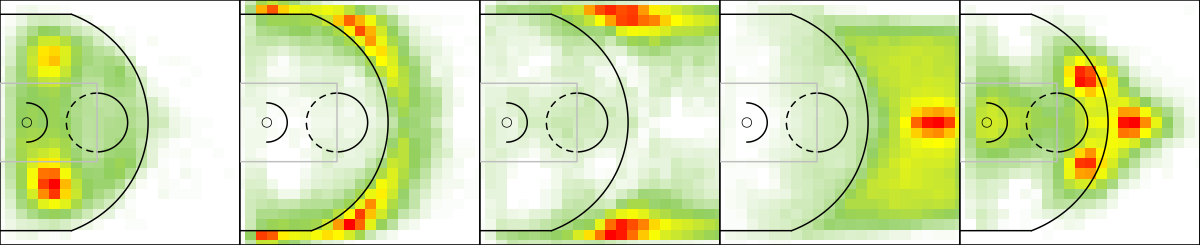
\includegraphics[width=0.7\textwidth]{graphics/H_bases}
\end{center}
\end{frame}

\begin{frame}{Inference}
``Partially Bayes'' estimation of all model parameters:
\pause
\begin{itemize}
\item Multiresolution transition models provide partial likelihood factorization \cite{cox1975note}.
\item All model parameters estimated using R-INLA software \cite{rue2009approximate, lindgren2011explicit}.
\end{itemize}
\pause
Distributed computing implementation:
\begin{itemize}
\item Preprocessing involves low-resource, highly parallelizable tasks.
\item Parameter estimation involves several CPU- and memory-intensive tasks.
\item Calculating EPV from parameter estimates involves low-resource, highly parallelizable tasks.
\end{itemize}
\end{frame}

\begin{frame}{New insights from basketball possessions}
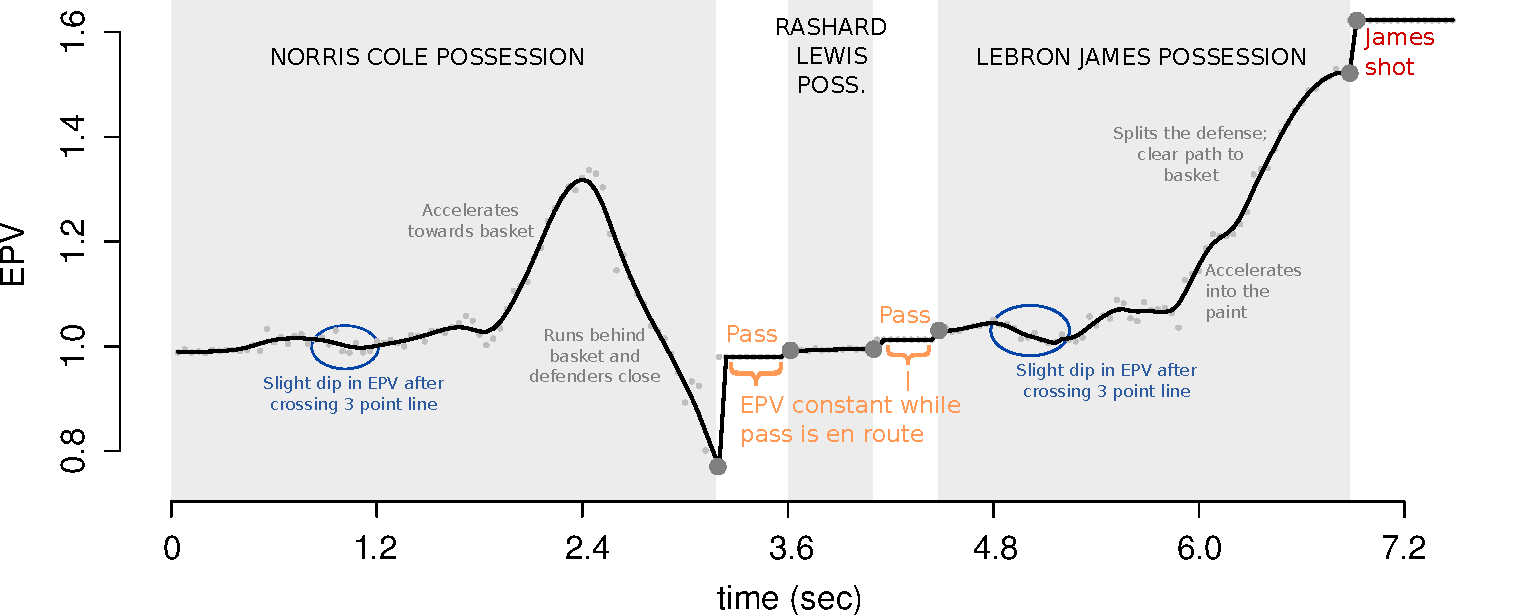
\includegraphics[width=1.0\textwidth]{graphics/ticker_1_edit}
\end{frame}

\begin{frame}{New insights from basketball possessions}
\begin{tabular}{ccc}
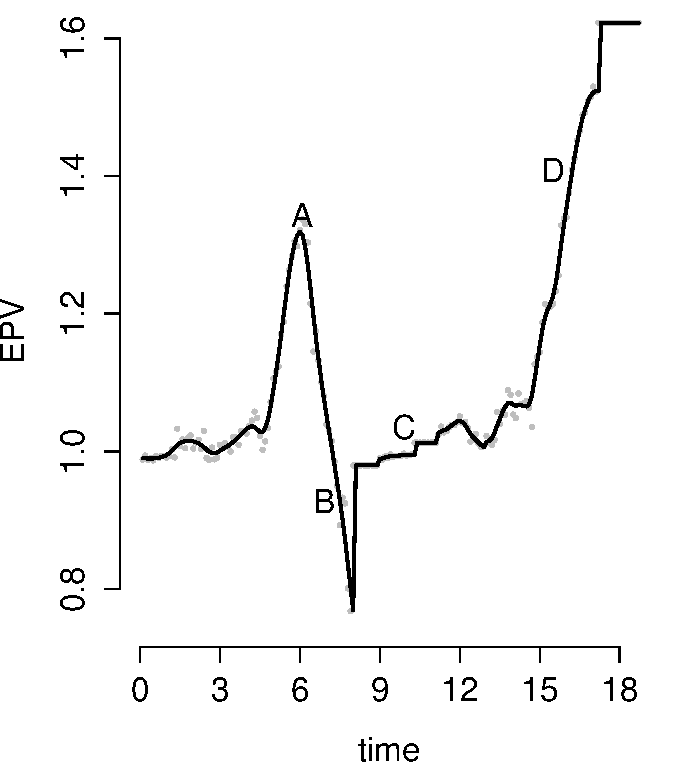
\includegraphics[width=0.3\textwidth]{graphics/ticker_2} & 
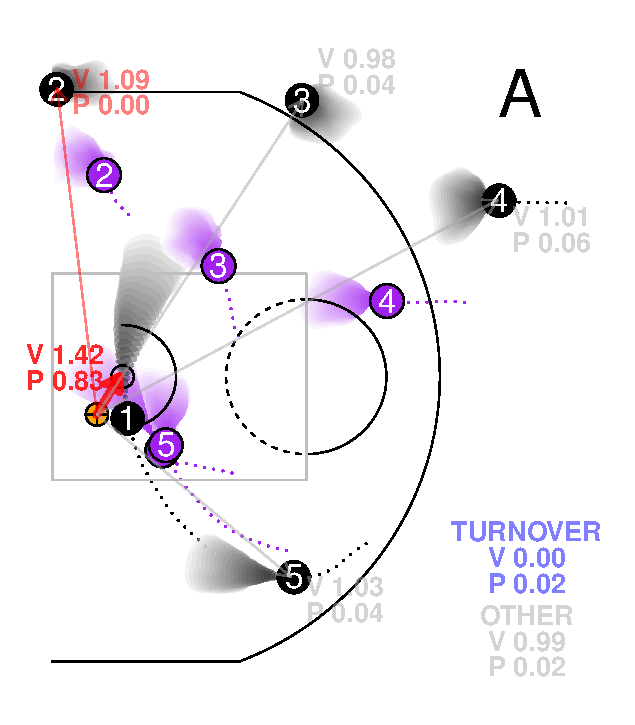
\includegraphics[width=0.3\textwidth]{graphics/micro_1_2} & 
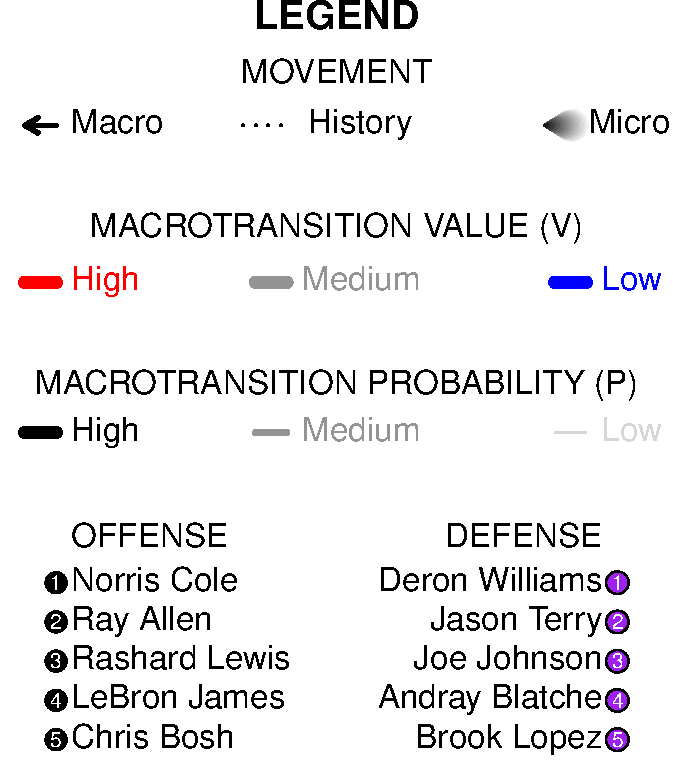
\includegraphics[width=0.3\textwidth]{graphics/legend} \\
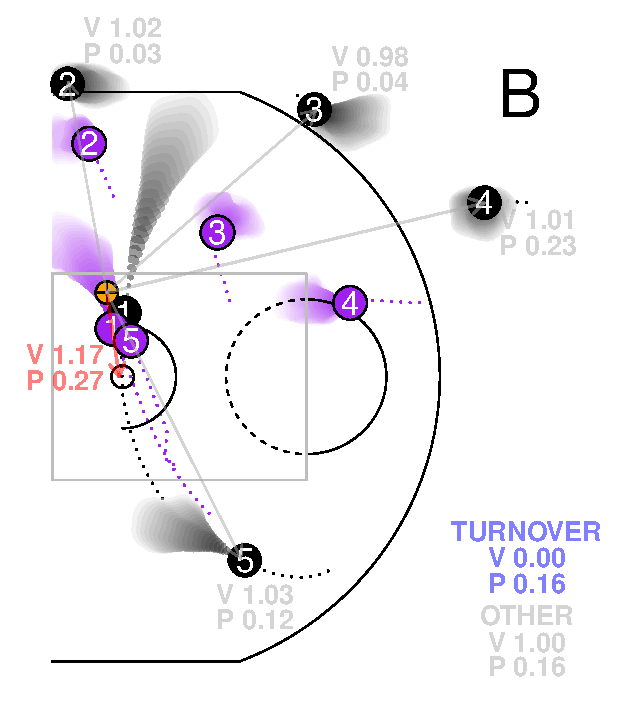
\includegraphics[width=0.3\textwidth]{graphics/micro_2_2} & 
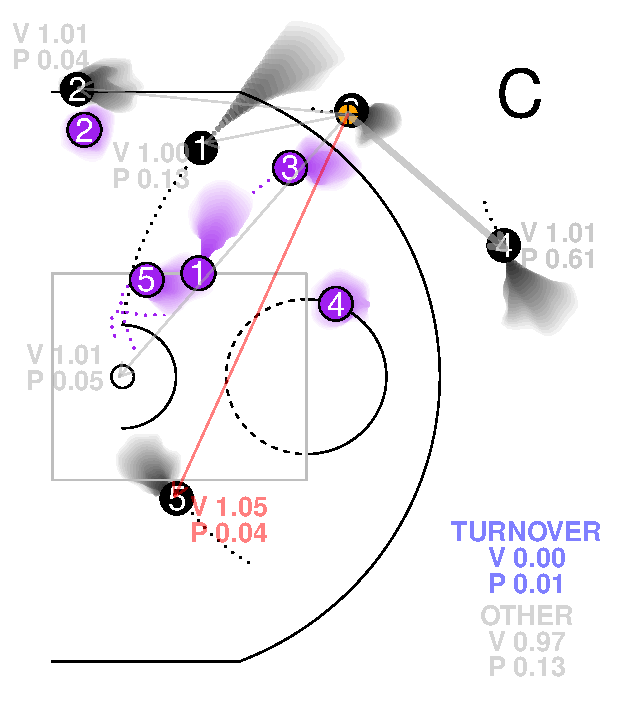
\includegraphics[width=0.3\textwidth]{graphics/micro_3_2} & 
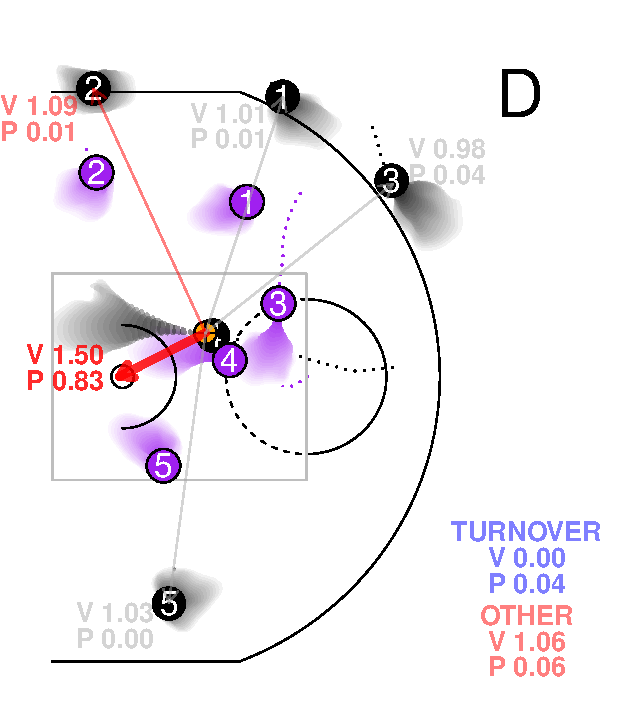
\includegraphics[width=0.3\textwidth]{graphics/micro_4_2} 
\end{tabular}
\end{frame}

\begin{frame}{New metrics for player performance}
EPV-added:
\begin{table}[ht]
\centering
\begin{tabular}{rlr}
  \toprule
Rank &  Player & EPVA \\
   \midrule
1 & Kevin Durant & 3.26 \\
2 & LeBron James & 2.96 \\
3 & Jose Calderon & 2.79 \\
4 & Dirk Nowitzki & 2.69 \\
5 & Stephen Curry & 2.50 \\
6 & Kyle Korver & 2.01 \\
7 & Serge Ibaka & 1.70 \\
8 & Channing Frye & 1.65 \\
9 & Al Horford & 1.55 \\
10 & Goran Dragic & 1.54 \\
\bottomrule
\end{tabular}
\quad
\begin{tabular}{rlr}
  \toprule
Rank & Player & EPVA \\ 
  \midrule
277 & Zaza Pachulia & -1.55 \\
278 & DeMarcus Cousins & -1.59 \\
279 & Gordon Hayward & -1.61 \\
280 & Jimmy Butler & -1.61 \\
281 & Rodney Stuckey & -1.63 \\
282 & Ersan Ilyasova & -1.89 \\
283 & DeMar DeRozan & -2.03 \\
284 & Rajon Rondo & -2.27 \\
285 & Ricky Rubio & -2.36 \\
286 & Rudy Gay & -2.59 \\
\bottomrule
\end{tabular}
\caption[]{Top 10 and bottom 10 players by EPV-added (EPVA) per game in 2013-14, minimum 500 touches during season.}
\end{table}
\end{frame}

\begin{frame}{New metrics for player performance}
Shot satisfaction:
\begin{table}[ht]
\centering
\begin{tabular}{rlr}
  \toprule
Rank &  Player & Satis. \\
   \midrule
1 & Mason Plumlee & 0.35 \\
2 & Pablo Prigioni & 0.31 \\
3 & Mike Miller & 0.27 \\
4 & Andre Drummond & 0.26 \\
5 & Brandan Wright & 0.24 \\
6 & DeAndre Jordan & 0.24 \\
7 & Kyle Korver & 0.24 \\
8 & Jose Calderon & 0.22 \\
9 & Jodie Meeks & 0.22 \\
10 & Anthony Tolliver & 0.22 \\
\bottomrule
\end{tabular}
\quad
\begin{tabular}{rlr}
\toprule
Rank & Player & Satis. \\ 
\midrule
277 & Garrett Temple & -0.02 \\
278 & Kevin Garnett & -0.02 \\
279 & Shane Larkin & -0.02 \\
280 & Tayshaun Prince & -0.03 \\
281 & Dennis Schroder & -0.04 \\
282 & LaMarcus Aldridge & -0.04 \\
283 & Ricky Rubio & -0.04 \\
284 & Roy Hibbert & -0.05 \\
285 & Will Bynum & -0.05 \\
286 & Darrell Arthur & -0.05 \\
\bottomrule
\end{tabular}
\caption[]{Top 10 and bottom 10 players by shot satisfaction in 2013-14, minimum 500 touches during season.}
\end{table}
\end{frame}

\begin{frame}{Acknowledgements and future work}
Our EPV framework can be extended to better incorporate unique basketball strategies:
\begin{itemize}
\item Additional macrotransitions can be defined, such as pick and rolls, screens, and other set plays.
\item Use more information in defensive matchups (only defender locations, not identities, are currently used).
\item Summarize and aggregate EPV estimates into useful player- or team-specific metrics.
\end{itemize}
\pause
Thanks to:
\begin{itemize}
\item Co-authors: Alex D'Amour, Luke Bornn, Kirk Goldsberry.
\item Colleagues: Alex Franks, Andrew Miller.
\end{itemize}
\end{frame}

%Let $M(t)$ be the event that a pass attempt, shot attempt, or turnover occurs in $(t, t + \epsilon]$.
%$$\prob(Z_{t + \epsilon} | \Fz_t) = \prob(Z_{t + \epsilon
%\textbf{Macrotransition model}

%ticktacky assumptions
%C_t is \Fz_t measureable 
%C_t semi-Markov
%\E[X|C_{\tau}, \Fz_t] = \E[X|C_{\tau_t}] if ballcarrier at t, else \E[X|\F_t] = \E[X| C_t]

\begin{frame}[allowframebreaks]
\frametitle{References}
\setbeamertemplate{bibliography item}{[\theenumiv]}
    \tiny{\bibliographystyle{apalike} }
    \bibliography{Refs}
\end{frame}

\end{document}
